	Experiments done in c-code are presented here. First the spectral behaviour of the multi-pass resampling method for an affine transform is checked. Then the new geometric method is compared to the Ripmap.

%On présente ici des expériences réalisées en C. On vérifie d'abord le comportement spectral du traitement multi-étape d'une affinité. On compare ensuite la nouvelle méthode au Ripmap.

\subsection{Multi-pass resampling method for an affine transform}

%\subsection{Décomposition multi-étapes d'une affinité}
 
 
 The results of multi-pass resampling method for an affine transform \cite{szeliski2010high} (part \ref{szeliski_section}) as well as the image's spectrum at the diffrents steps are shown in this section. The affine transform being here a shear, the decompostion turn into three basic steps, instead of four ones for a general affine transform.  
 
 %On présente ici les résultats de la décomposition multi-étapes d'une affinité \cite{szeliski2010high} (section \ref{szeliski_section}), ainsi que le spectre de l'image aux différentes étapes. L'affinité utilisée étant elle-même un \emph{shear}, la décomposition se réduit à trois étapes élémentaires, au lieu des quatres d'une affinité quelconque.
 \begin{figure}
		\centering
		\subfigure[Initial image (scale 3/8)]{
			{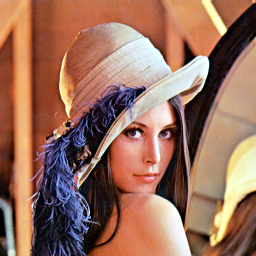
\includegraphics[scale=0.375]{decompoSzeliski_sinc_image_entree.png}}
			{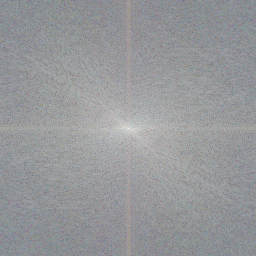
\includegraphics[scale=0.375]{decompoSzeliski_sinc_fourier_entree.png}}
		}
		\subfigure[Inital image in a nine times larger one (scale 1/8)]{
			{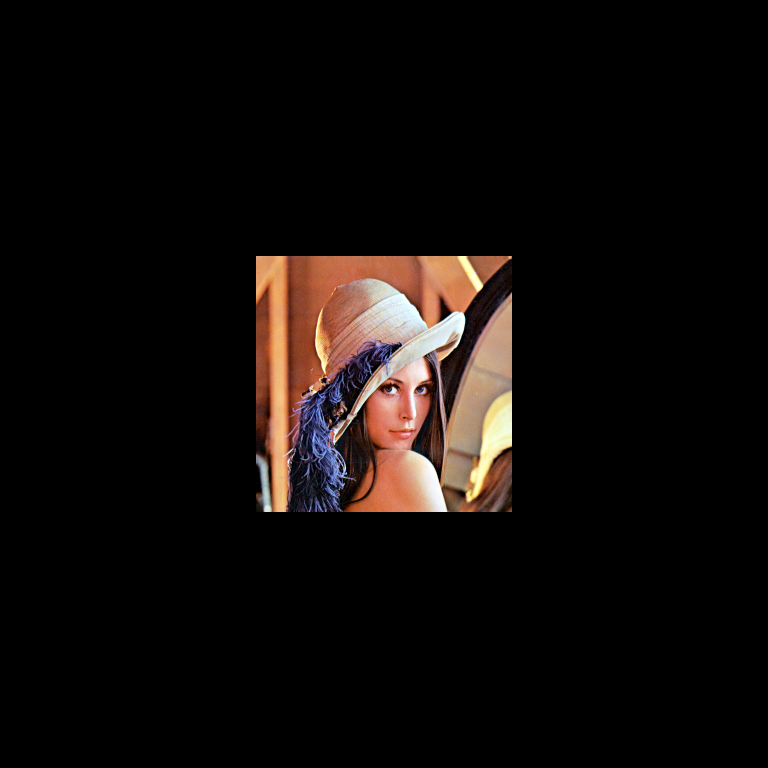
\includegraphics[scale=0.125]{decompoSzeliski_sinc_image1.png}}
			{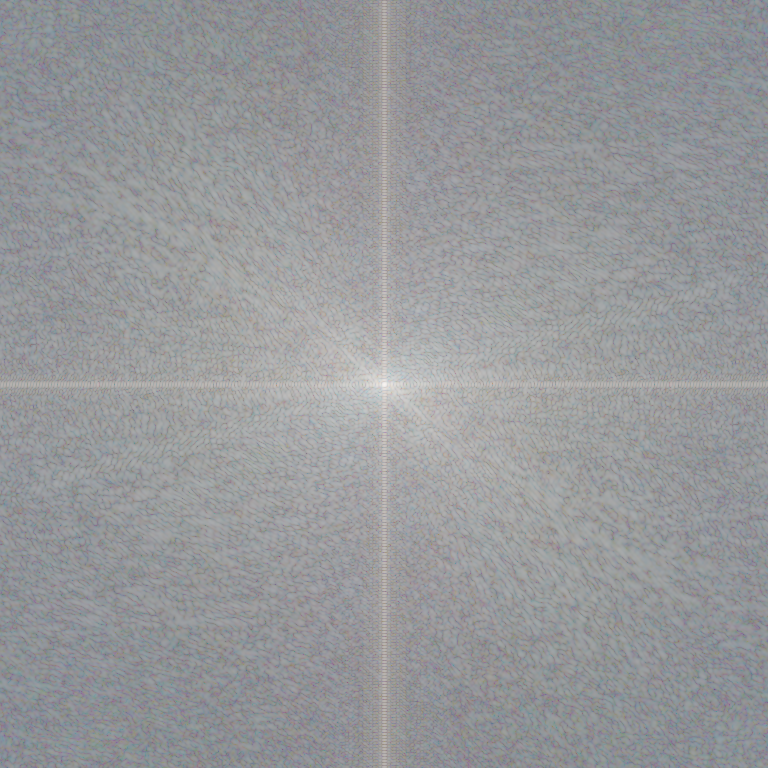
\includegraphics[scale=0.125]{decompoSzeliski_sinc_fourier1.png}}
		}
		\subfigure[After the first $\mathcal R$ (scale 1/8)]{
			{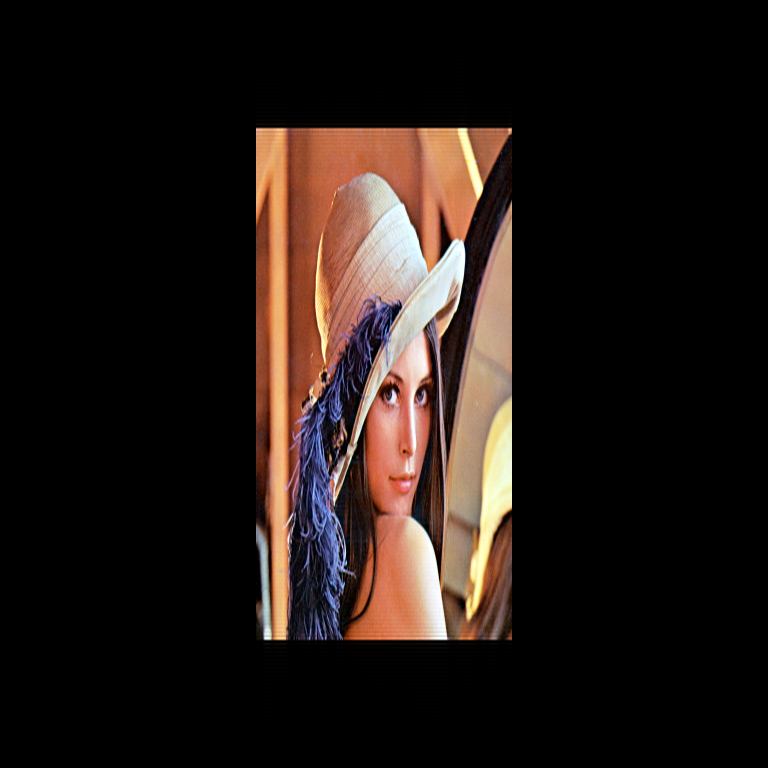
\includegraphics[scale=0.125]{decompoSzeliski_sinc_image2.png}}
			{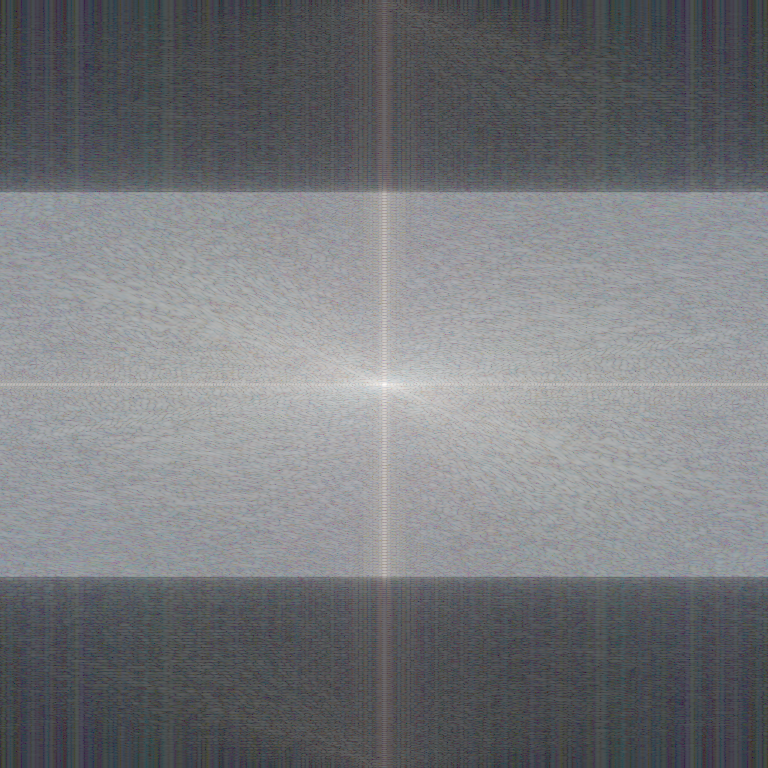
\includegraphics[scale=0.125]{decompoSzeliski_sinc_fourier2.png}}
		}
		\subfigure[After the second $\mathcal R$ (scale 1/8)]{
			{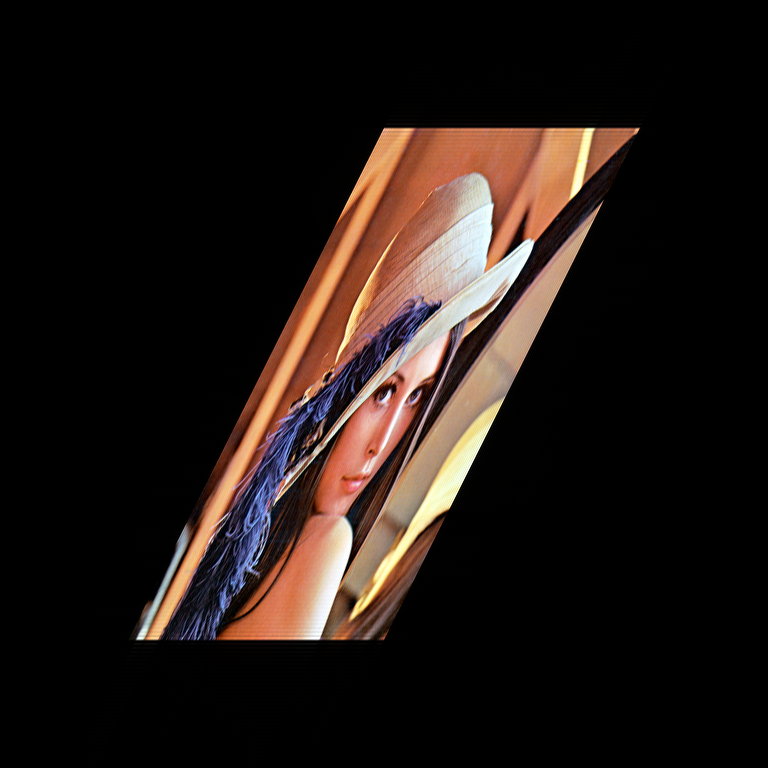
\includegraphics[scale=0.125]{decompoSzeliski_sinc_image3.png}}
			{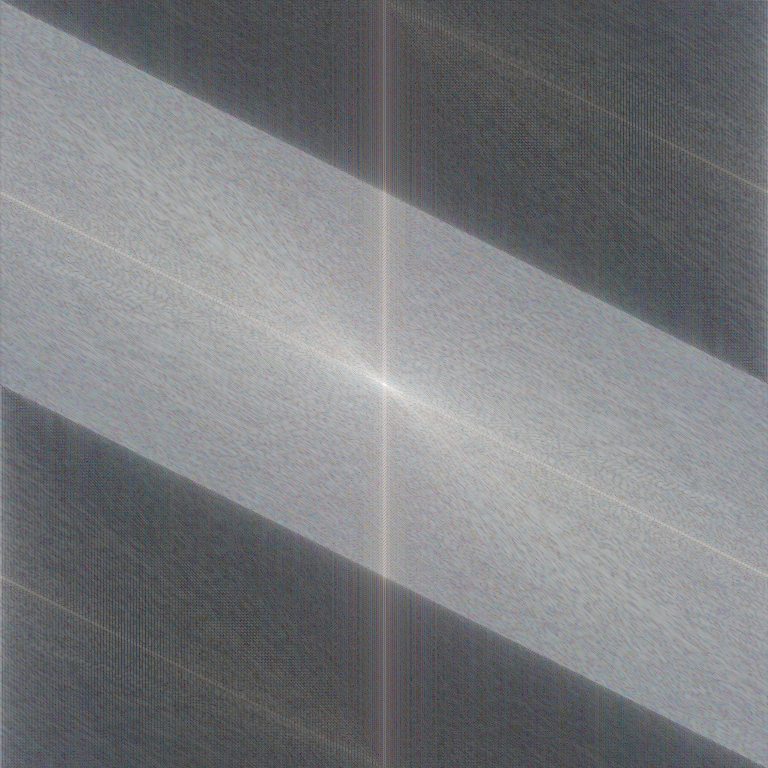
\includegraphics[scale=0.125]{decompoSzeliski_sinc_fourier3.png}}
		}
		\subfigure[After the third $\mathcal R$ (scale 1/8)]{
			{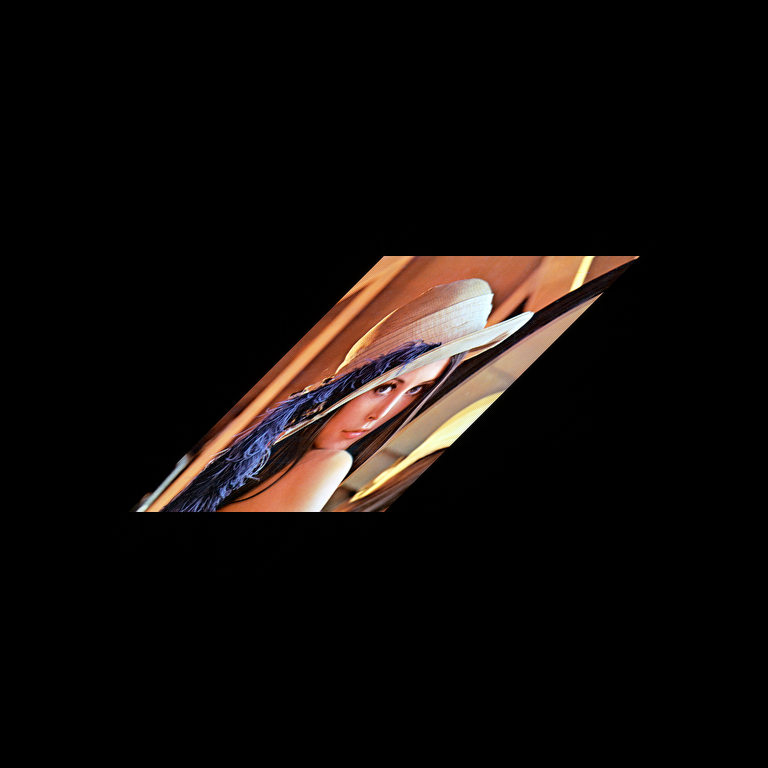
\includegraphics[scale=0.125]{decompoSzeliski_sinc_image4.png}}
			{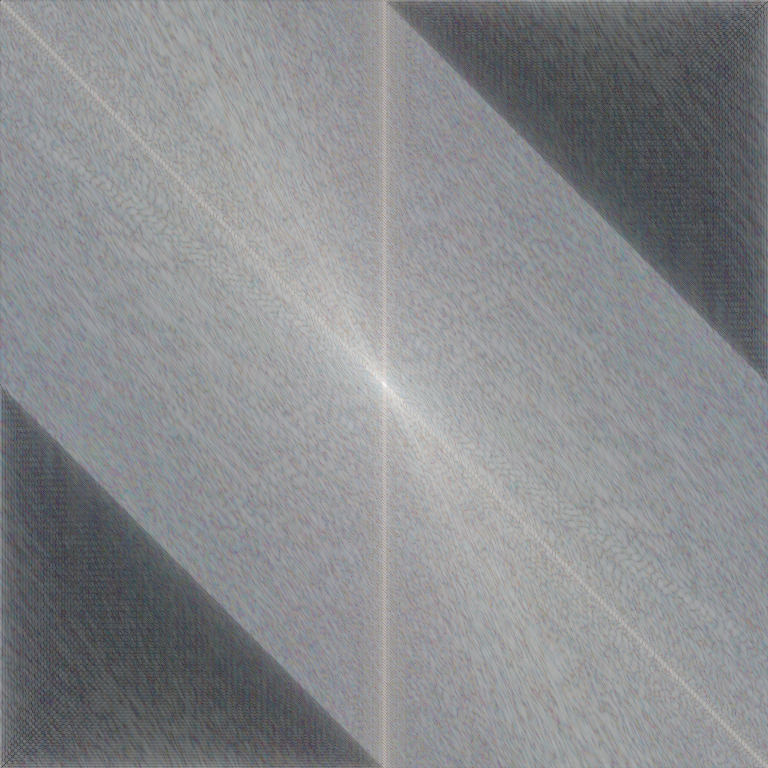
\includegraphics[scale=0.125]{decompoSzeliski_sinc_fourier4.png}}
		}
		\subfigure[Final image (scale 3/8)]{
			{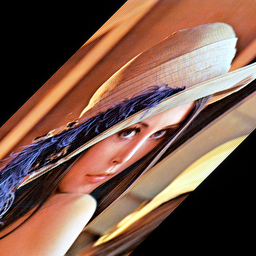
\includegraphics[scale=0.375]{decompoSzeliski_sinc_image_sortie.png}}
			{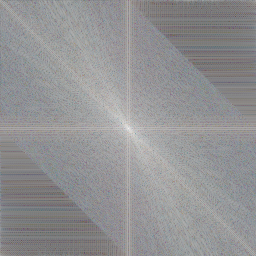
\includegraphics[scale=0.375]{decompoSzeliski_sinc_fourier_sortie.png}}
		}
		\caption{Steps of the multi-pass resampling method for an affine transform explained in \ref{szeliski_section} (on the left is the image at each steps, on the right is the logarithm of the modulus of the Fourier transform of this image). The interpolation filter is a sinc function (of period 1)}
		\label{experiments_decompoSzeliski_sinc}
	\end{figure}
	%\begin{figure}
	%	\centering
	%	\subfigure[Image initiale (échelle 3/8)]{
	%		{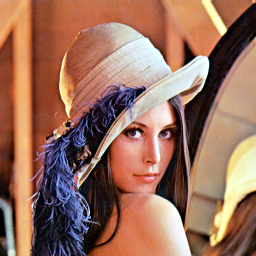
\includegraphics[scale=0.375]{decompoSzeliski_sinc_image_entree.png}}
	%		{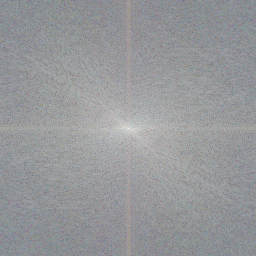
\includegraphics[scale=0.375]{decompoSzeliski_sinc_fourier_entree.png}}
	%	}
	%	\subfigure[Image plongée dans une image neuf fois plus grande (échelle 1/8)]{
	%		{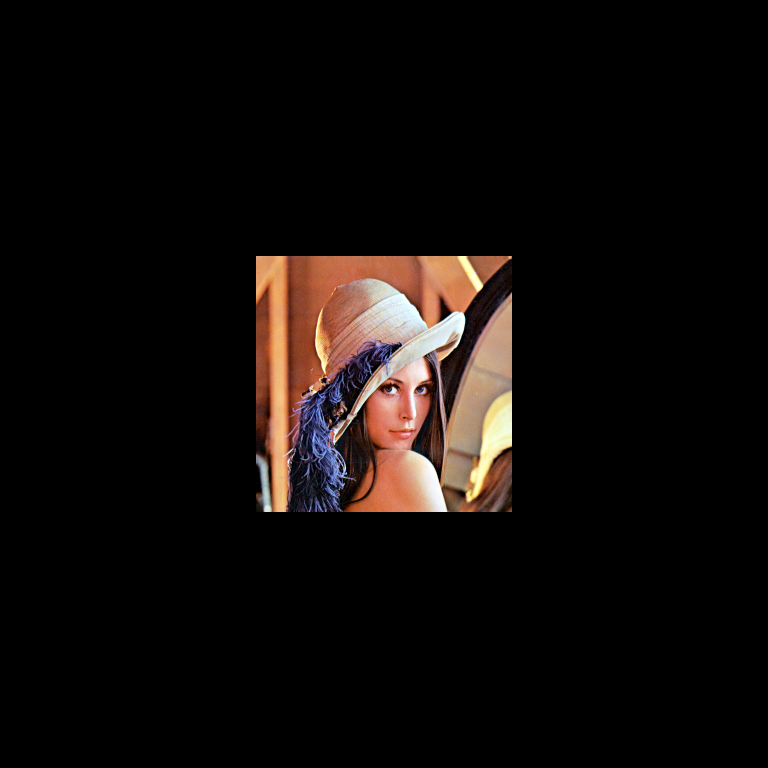
\includegraphics[scale=0.125]{decompoSzeliski_sinc_image1.png}}
	%		{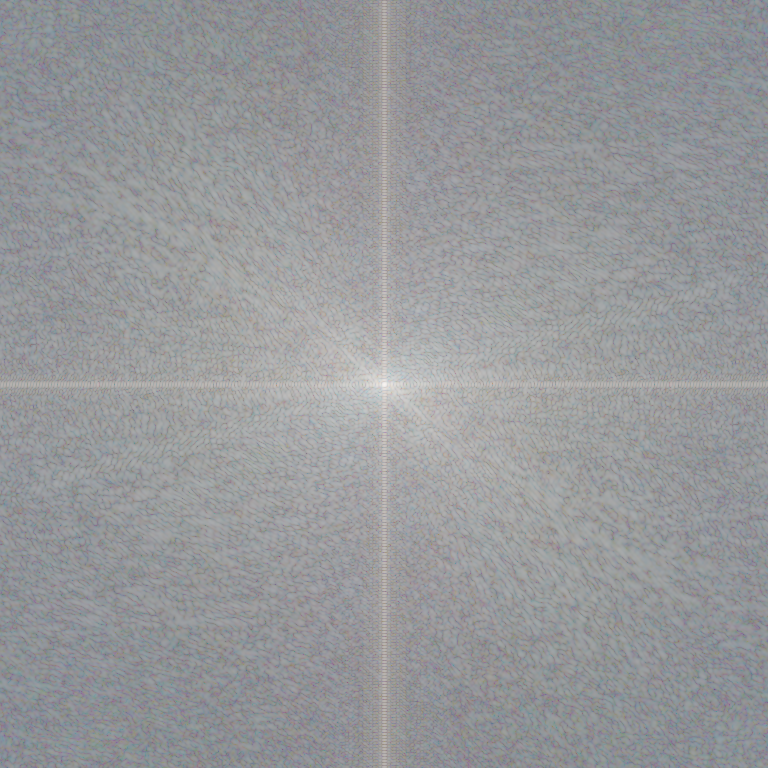
\includegraphics[scale=0.125]{decompoSzeliski_sinc_fourier1.png}}
	%	}
	%	\subfigure[Après le premier $\mathcal R$ (échelle 1/8)]{
	%		{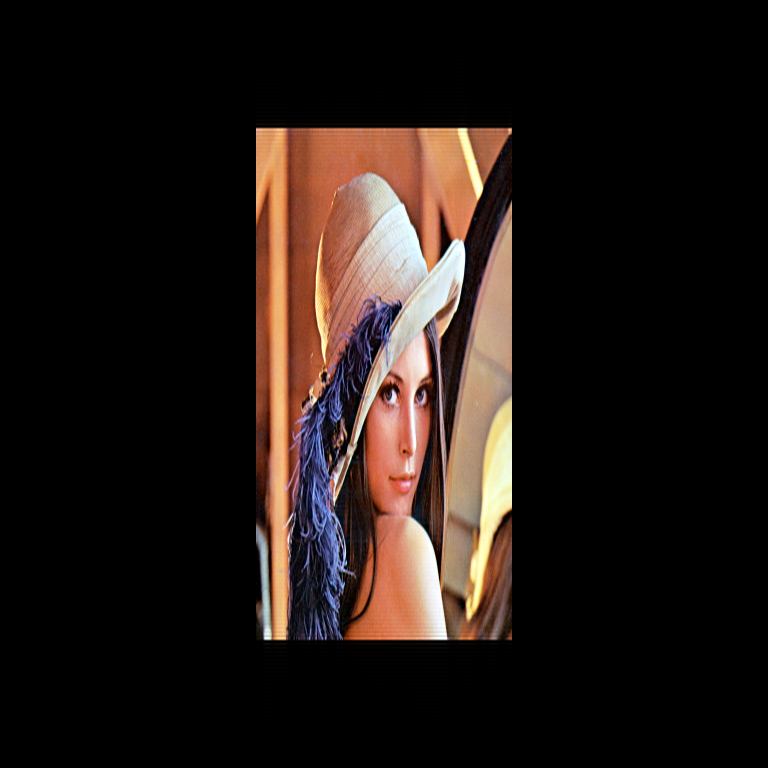
\includegraphics[scale=0.125]{decompoSzeliski_sinc_image2.png}}
	%		{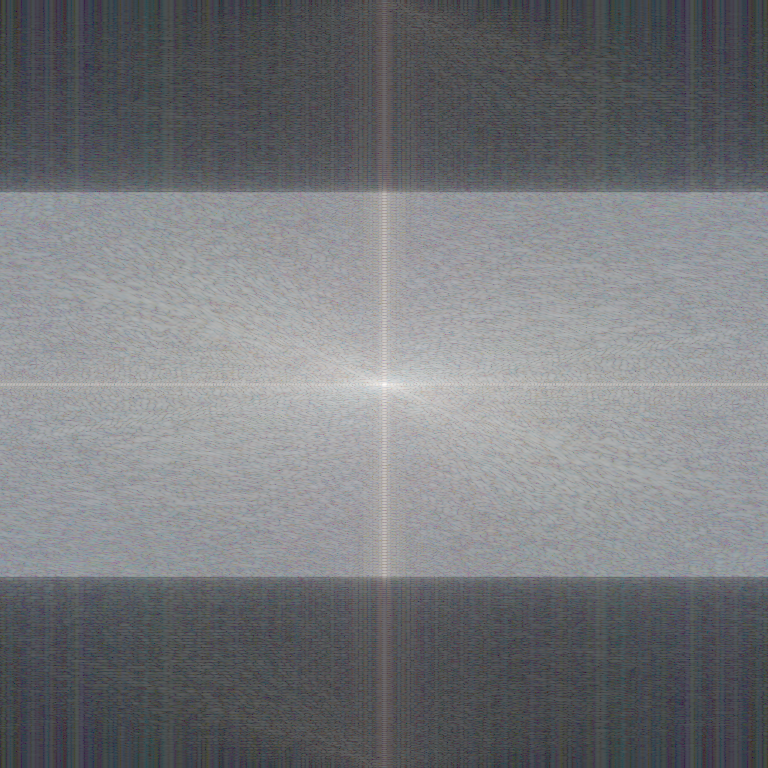
\includegraphics[scale=0.125]{decompoSzeliski_sinc_fourier2.png}}
	%	}
	%	\subfigure[Après le deuxième $\mathcal R$ (échelle 1/8)]{
	%		{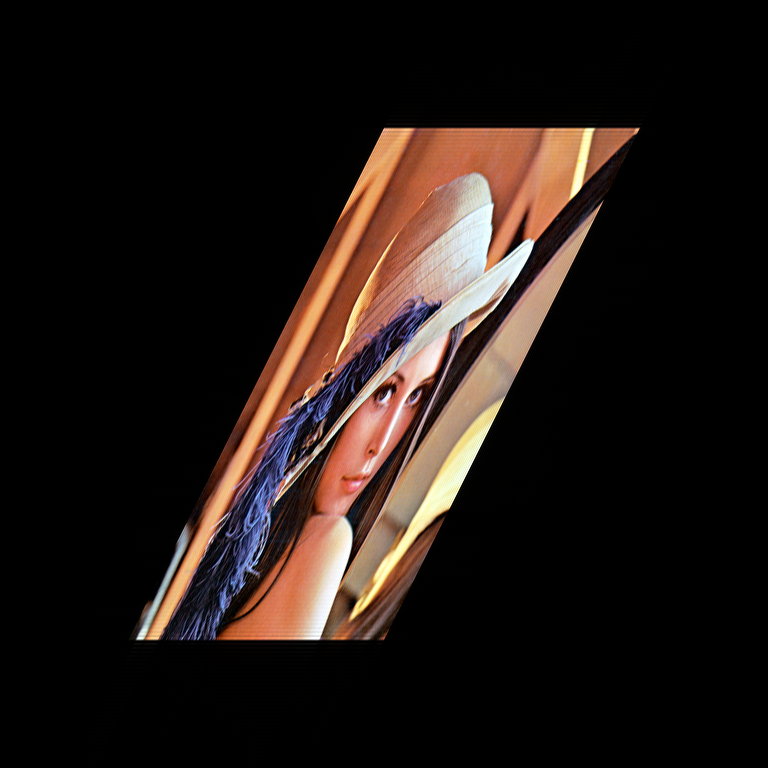
\includegraphics[scale=0.125]{decompoSzeliski_sinc_image3.png}}
	%		{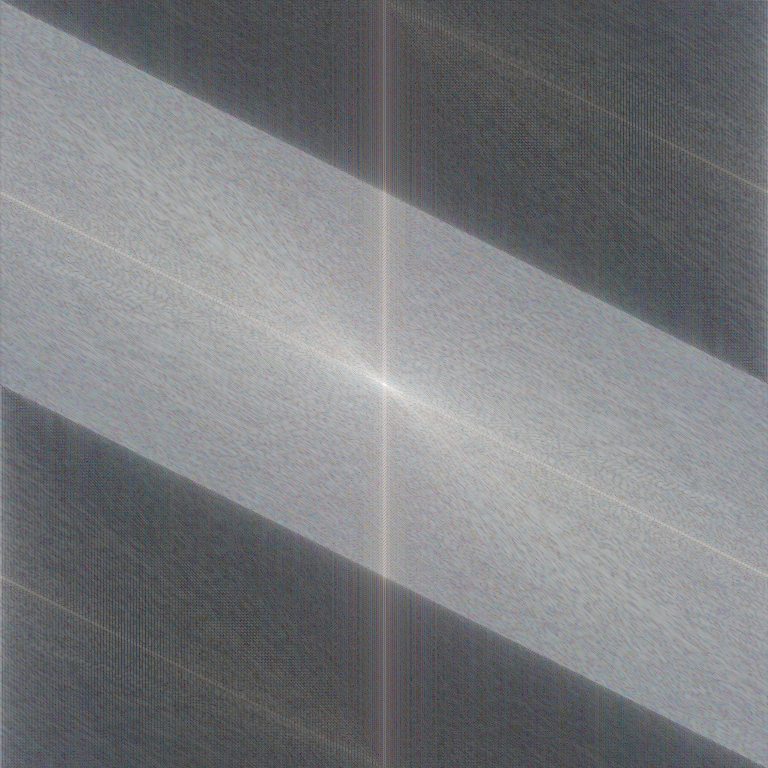
\includegraphics[scale=0.125]{decompoSzeliski_sinc_fourier3.png}}
	%	}
	%	\subfigure[Après le troisième $\mathcal R$ (échelle 1/8)]{
	%		{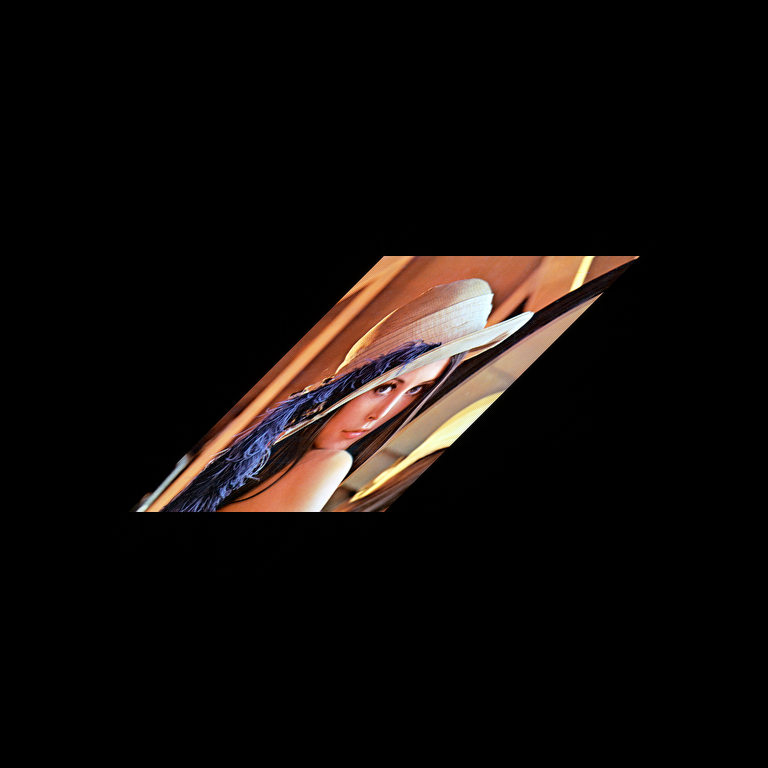
\includegraphics[scale=0.125]{decompoSzeliski_sinc_image4.png}}
	%	}
	%	\subfigure[Image finale (échelle 3/8)]{
	%		{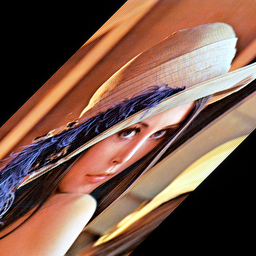
\includegraphics[scale=0.375]{decompoSzeliski_sinc_image_sortie.png}}
	%		{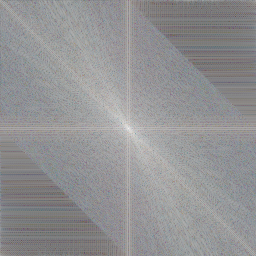
\includegraphics[scale=0.375]{decompoSzeliski_sinc_fourier_sortie.png}}
	%	}
	%	\caption{Étapes du traitement des affinités présenté en \ref{szeliski_section} (à gauche l'image à chaque étape, à droite le logarithme du module de la transformée de Fourier de cette image). Le filtre d'interpolation est un \emph{sinc} (de période 1)}
	%	\label{experiments_decompoSzeliski_sinc}
	%\end{figure}
	
	En figure \ref{experiments_decompoSzeliski_sinc}, le filtre utilisé est un \emph{sinc}, correspondant au \emph{raised cosine-weighted sinc} avec $\beta = 0$ ; pour rappel, le filtre a pour forme
	\[h : x \mapsto \sinc(\frac{x}{T})\frac{\cos(\frac{\pi\beta x}{T})}{1-\frac{4\beta^2x^2}{T^2}}\]
	On ne perd pas en qualité visuelle en réduisant la convolution à un nombre fini de termes suffisamment grand.
	
	Avec un $\beta$ plus élevé, on conserve des hautes fréquences sur l'extérieur du spectre, mais leur impact est faible quand l'image reprend sa taille initiale ; en augmentant $\beta$ (figure \ref{experiments_decompoSzeliski}), on peut donc autoriser un peu plus de repliement du spectre, en veillant à ce que visuellement, on n'observe aucun artefact. Comme l'augmentation de $\beta$ augmente la vitesse à laquelle le filtre décroit, on peut alors convoler sur des supports plus réduits, et donc gagner du temps. Avec $\beta = 0.36$, on peut restreindre la convolution à une somme de fneu termes (figure \ref{szeliski_plotRaisedCosine}) (neuf est le nombre de termes de base ; il est plus grand lors des sur-échantillonnages car le support du filtre de convolution est adaptatif). Cette valeur $\beta = 0.36$ est celle qu'on utilise pour les autres expériences.
 
	\begin{figure}
		\centering
		\subfigure[Image initiale (échelle 3/8)]{
			{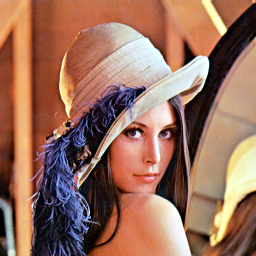
\includegraphics[scale=0.375]{decompoSzeliski_image_entree.png}}
			{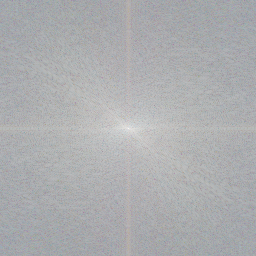
\includegraphics[scale=0.375]{decompoSzeliski_fourier_entree.png}}
		}
		\subfigure[Image plongée dans une image neuf fois plus grande (échelle 1/8)]{
			{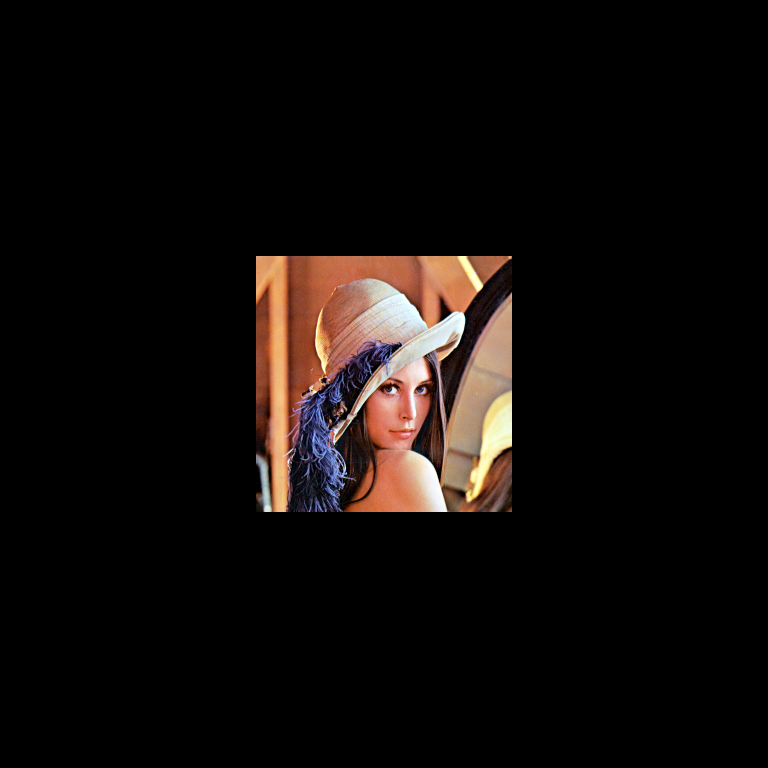
\includegraphics[scale=0.125]{decompoSzeliski_image1.png}}
			{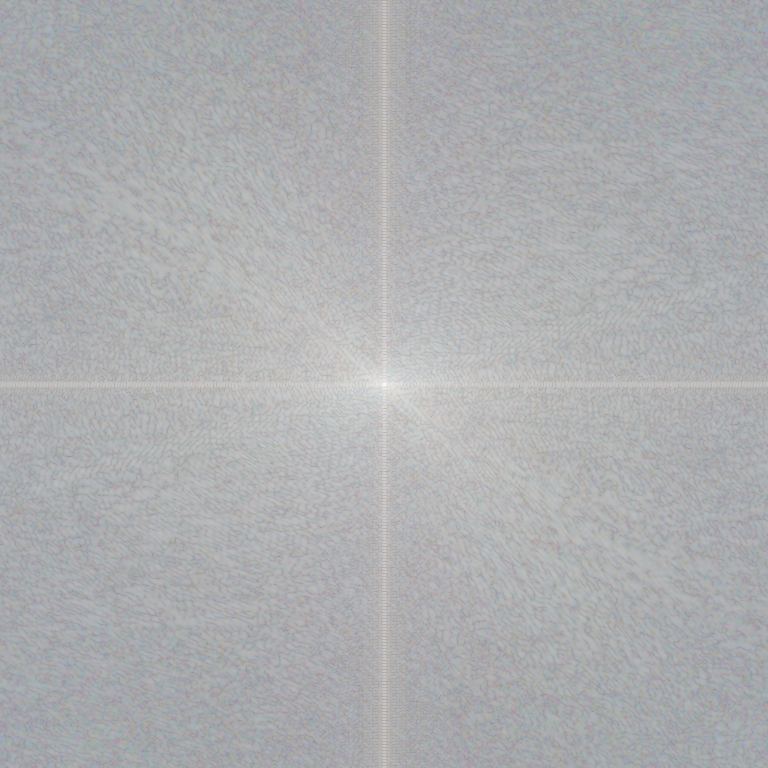
\includegraphics[scale=0.125]{decompoSzeliski_fourier1.png}}
		}
		\subfigure[Après le premier $\mathcal R$ (échelle 1/8)]{
			{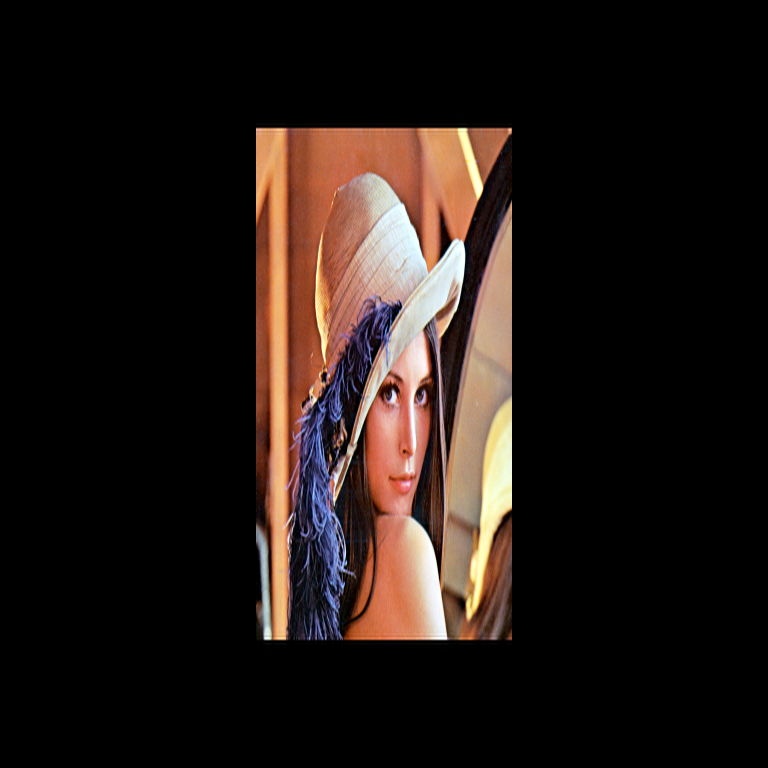
\includegraphics[scale=0.125]{decompoSzeliski_image2.png}}
			{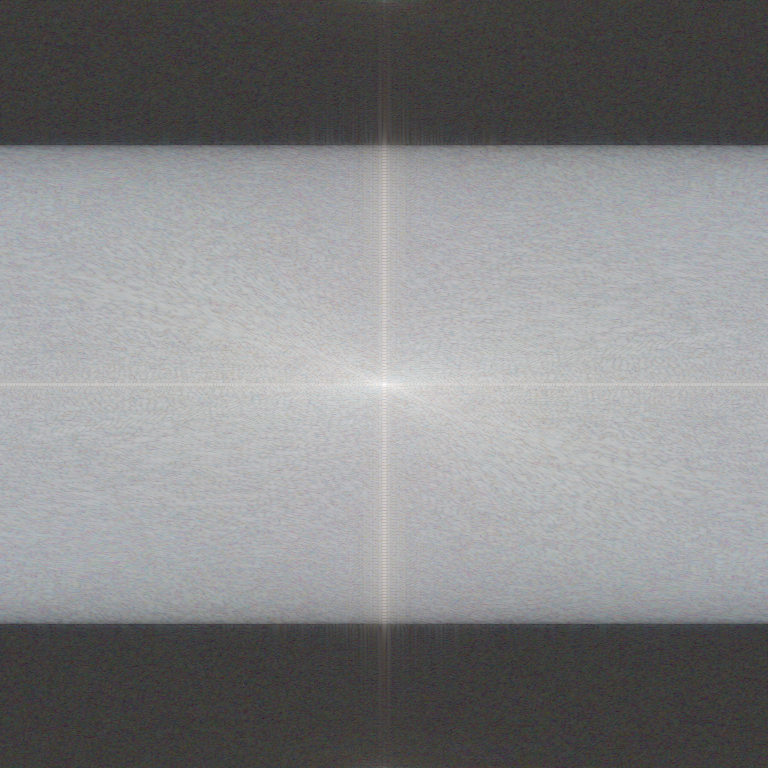
\includegraphics[scale=0.125]{decompoSzeliski_fourier2.png}}
		}
		\subfigure[Après le deuxième $\mathcal R$ (échelle 1/8)]{
			{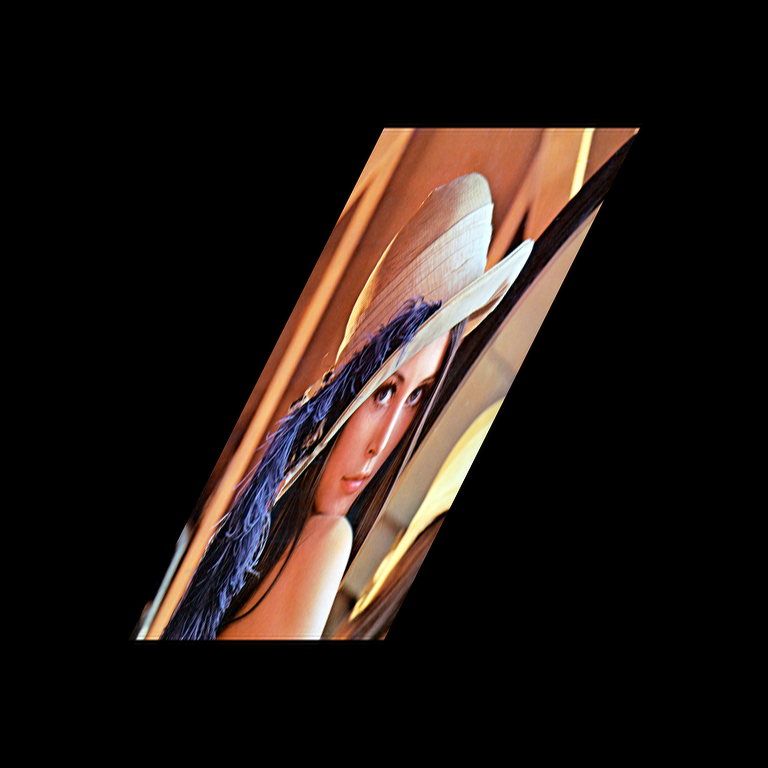
\includegraphics[scale=0.125]{decompoSzeliski_image3.png}}
			{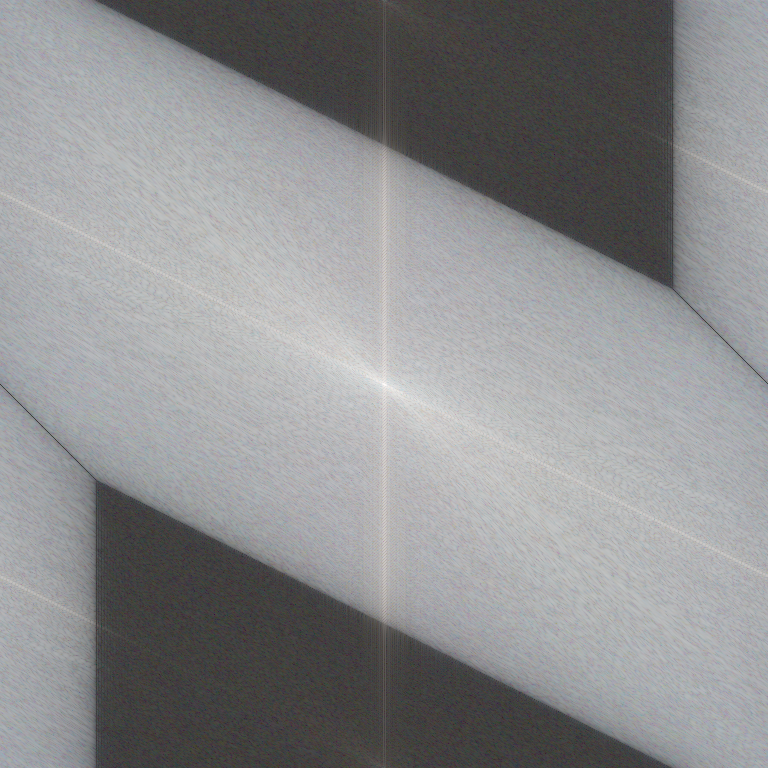
\includegraphics[scale=0.125]{decompoSzeliski_fourier3.png}}
		}
		\subfigure[Après le troisième $\mathcal R$ (échelle 1/8)]{
			{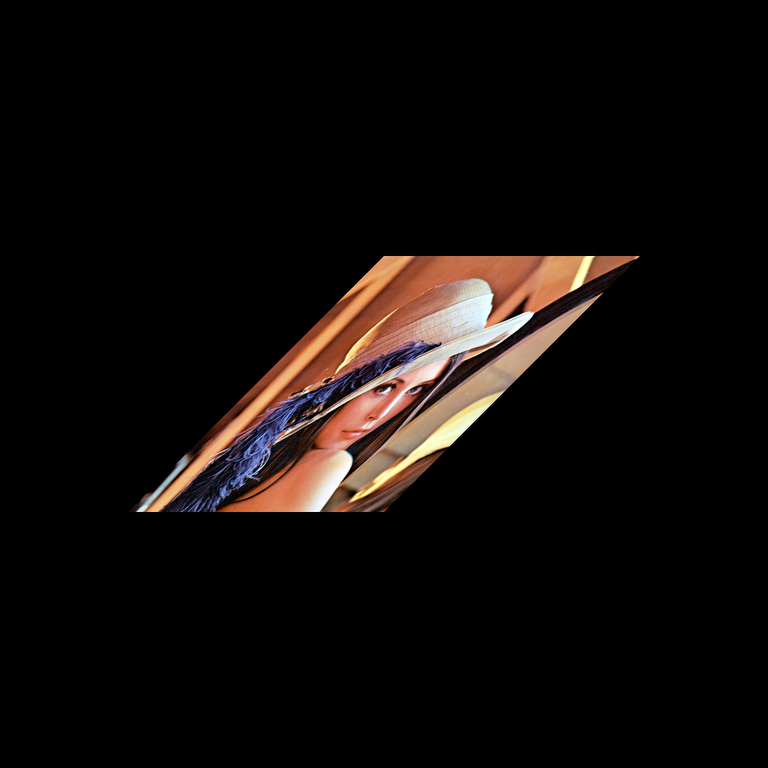
\includegraphics[scale=0.125]{decompoSzeliski_image4.png}}
			{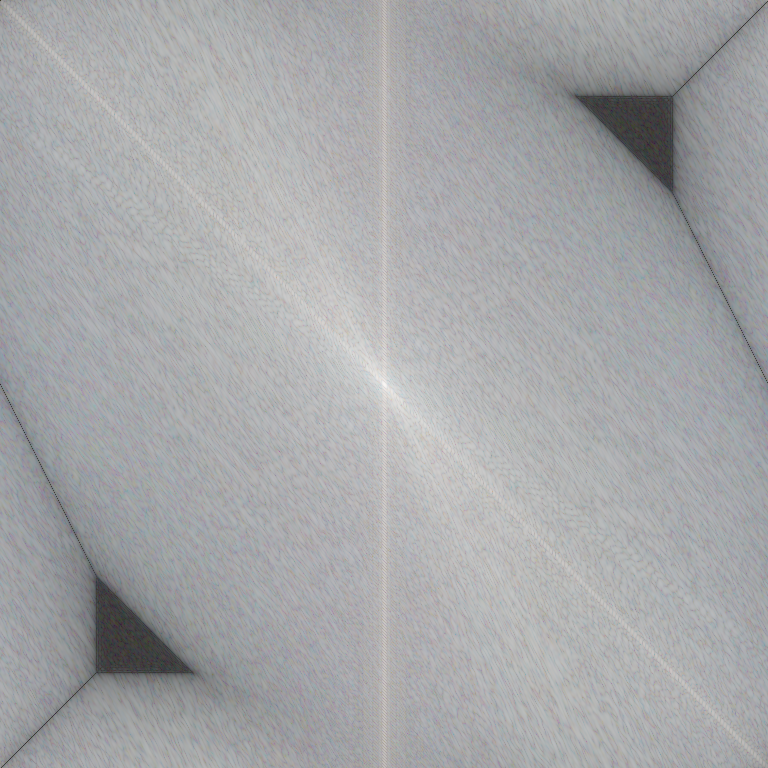
\includegraphics[scale=0.125]{decompoSzeliski_fourier4.png}}
		}
		\subfigure[Image finale (échelle 3/8)]{
			{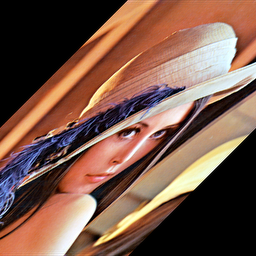
\includegraphics[scale=0.375]{decompoSzeliski_image_sortie.png}}
			{
\includegraphics[scale=0.375]{decompoSzeliski_fourier_sortie.png}}
		}
		\caption{Étapes du traitement des affinités présenté en \ref{szeliski_section} (à gauche l'image à chaque étape, à droite le logarithme du module de la transformée de Fourier de cette image). Le filtre d'interpolation est un \emph{raised cosine-weighted sinc} (de période 1, de \emph{roll-off factor} $\beta = 0.25$)}
		\label{experiments_decompoSzeliski}
	\end{figure}
